\section{Learning a default strategy}
\label{sec:part2}
In the previous chapter we created a calculator that can determine the strength of a hand by calculating the probability of winning. In this chapter we shall use this calculator in the process of developing a strategy for the APC.

When the APC first joins a poker game it has no information about the opponents, and in this case it must use a default strategy while it gathers more information.

In this chapter we will find a solution to the problem statement:

\vspace{4mm}
\begin{statementBox2}{Problem statement 2}
How can we develop a default strategy for APC without having information about the playing style of the opponents?
\end{statementBox2}
\vspace{4mm}

Even though players have different strategies they often have some decisions in common. Most players tend to play more aggressively the stronger their hand are the bigger are their chances of winning and likewise most players will play defensive or fold if they have a weak hand. These tendencies can be used in a default strategy. The popular decisions are more likely to be good. For instance, most players agree that it is unwise to fold a pair of aces in the pre-flop. 

The default strategy has to work against every strategy, therefore it is impossible for it to be better than all of them. The goal for the default strategy is not to win, although that is preferable, but instead to reduce the loses while it gathers information about the opponent.

\subsection{Design}
To develop a strategy in poker the two most commonly used options are to either directly program the procedures in the code or to create an algorithm that can learn a strategy from a player. 

Programming the procedures in the code requires the programmer to have a deep insight in how to play poker and how to make the optimal decisions during a game. One can also use the expertise of professional poker players in case one lacks the insight.

The algorithm uses the concept watch and learn by observing other players and learn the strategy behind their decisions. This method requires that the algorithm has someone to observe.

Since we do not have any particular insight in how to play poker and do not have expertise from a professional poker player, we will implement an algorithm. Additionally, by using this method the computer is not limited by our understanding of the game. 

We will use data from real life poker games for the algorithm. The data is further described in section \ref{sec:default-test}.\\

To implement the algorithm we use an artificial neural network (ANN), see section \ref{sec:nn}. The ANN is well suited for finding patterns of the players decisions. 

The total network error (TNE) is how great a deviation there is from the expected output to the actual output of the ANN. Our goal is to design an ANN with a TNE of five percent or less. We find five percent to be acceptable as players often take irrational decisions and the ANN only tries to find an approximation of the results. 

We use an iterative development method to design the ANN. We start by designing a simple ANN and then move on to more complex ANN's.\\

All our ANN's have exactly two outputs. The first output is whether or not to be defensive by checking or calling and the second output is whether or not to be aggressive by betting or raising. The closer an output is to the value one, the more certain the ANN is, that it is the correct decision. 

All our ANN's use normalised inputs, weighted sum as input function, and a sigmoid function as transfer function. The reason we settle for a sigmoid function rather than a step function is because the sigmoid function allows us to see how certain the ANN is of each decision being correct.

The ANN's uses backpropagation for learning with a learning rule of 0,2.

\subsection{Artificial neural network}
\label{sec:nn}
An ANN is inspired by the human brain. It can be used for pattern recognition or classification among other things. An ANN can take any number of inputs and return any number of outputs. 

An ANN is made up of neurons that are connected into a network. Each neuron takes a set of inputs and returns a single output. The output of a neuron is sent as an input to all the connected neurons. Each input has a weight that determines influence of the input. The neuron uses an input function to calculate the net input, usually the sum of all weighted inputs, and pass it on to the transfer function. The type of transfer function determines the output. A step function returns zero or one if the net input is above a certain threshold. This is useful for logical functions. If one needs a value between zero and one a sigmoidal function can be used instead.

Figure \ref{fig:neuron} models a neuron. Here the weighted inputs $w_{i1}$, $w_{i2}$, and $w_{i3}$ are all sent to the input function $\sum$ which then calculates the net input $net_{i}$. The transfer function $f$ then calculates the output from the net input.

\begin{figure}[H]
  \center
    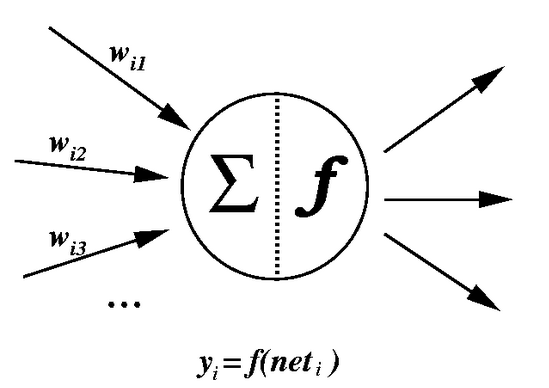
\includegraphics[scale=0.4]{images/nn/neuron.png}
  \caption{Model of a neuron.\cite{neuron} \label{fig:neuron}}
\end{figure}

The neurons in an ANN are distributed in layers as shown in figure \ref{fig:perceptron} and \ref{fig:mlp}. The coloured circles represents neurons and the arrows represents the connections between the neurons. There are three layers, an input layer, a hidden layer, and an output layer. An ANN consists of one input layer and one output layer but may contain any number of hidden layers. The simplest type of ANN is the perceptron which has no hidden layers, see figure \ref{fig:perceptron}. It is used for single calculations. A multilayer perceptron is another type of ANN which contains hidden layers. It is used for more complex domains with multiple layers of computations. The number of hidden neurons indicates the number of calculations. A multilayer perceptron is illustrated in figure 6.

\def\layersep{2.5cm}

\begin{figure}[H]
\center
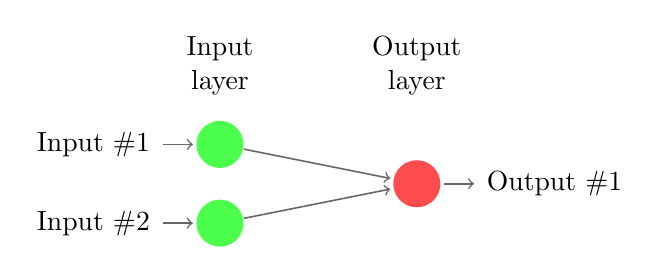
\begin{tikzpicture}[shorten >=1pt,->,line width=0.2mm,draw=black!60, node distance=\layersep]
    \tikzstyle{every pin edge}=[<-,shorten <=1pt]
    \tikzstyle{neuron}=[circle,fill=black!25,minimum size=17pt,inner sep=0pt]
    \tikzstyle{input neuron}=[neuron, fill=green!70];
    \tikzstyle{output neuron}=[neuron, fill=red!70];
    \tikzstyle{hidden neuron}=[neuron, fill=blue!70];
    \tikzstyle{annot} = [text width=4em, text centered]

    % Draw the input layer nodes
    \node[input neuron, pin=left:Input \#1] (I-1) at (0,-1) {};
    \node[input neuron, pin=left:Input \#2] (I-2) at (0,-2) {};

    % Draw the output layer node
    \node[output neuron,pin={[pin edge={->}]right:Output \#1}] (O-1) at (\layersep,-1.5) {};

    % Connect every node in the input layer with every node in the
    % hidden layer.
    \path (I-1) edge (O-1);
    \path (I-2) edge (O-1);

    % Annotate the layers
    \node[annot,above of=I-1, node distance=1cm] (il) {Input layer};
    \node[annot,right of=il] {Output layer};
\end{tikzpicture}
\caption{Perceptron with two inputs and one output. \label{fig:perceptron}}
\end{figure}
\vspace{4mm}
\def\layersep{2.5cm}

\begin{figure}[H]
\center
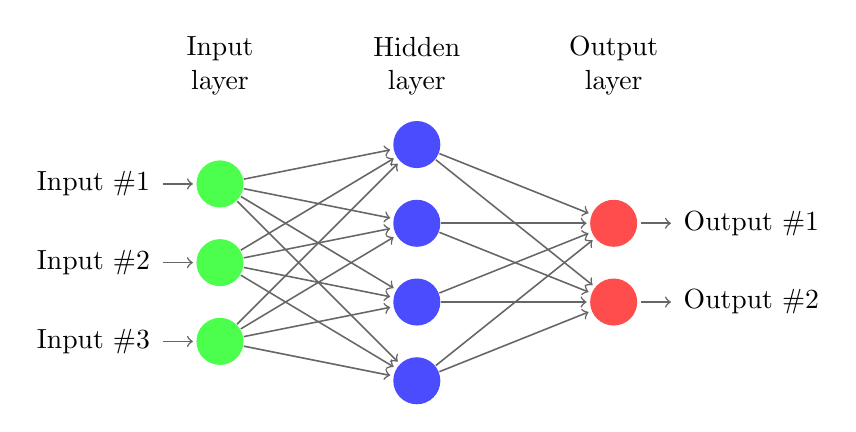
\begin{tikzpicture}[shorten >=1pt,->,line width=0.2mm,draw=black!60, node distance=\layersep]
    \tikzstyle{every pin edge}=[<-,shorten <=1pt]
    \tikzstyle{neuron}=[circle,fill=black!25,minimum size=17pt,inner sep=0pt]
    \tikzstyle{input neuron}=[neuron, fill=green!70];
    \tikzstyle{output neuron}=[neuron, fill=red!70];
    \tikzstyle{hidden neuron}=[neuron, fill=blue!70];
    \tikzstyle{annot} = [text width=4em, text centered]

    % Draw the input layer nodes
    %\foreach \name / \y in {1,...,4}
    % This is the same as writing \foreach \name / \y in {1/1,2/2,3/3,4/4}
    \node[input neuron, pin=left:Input \#1] (I-1) at (0,-1.5) {};
    \node[input neuron, pin=left:Input \#2] (I-2) at (0,-2.5) {};
    \node[input neuron, pin=left:Input \#3] (I-3) at (0,-3.5) {};

    % Draw the hidden layer 1 nodes
    \node[hidden neuron] (H-1) at (\layersep,-1) {};
    \node[hidden neuron] (H-2) at (\layersep,-2) {};
    \node[hidden neuron] (H-3) at (\layersep,-3) {};
    \node[hidden neuron] (H-4) at (\layersep,-4) {};

    % Draw the output layer node
    \node[output neuron,pin={[pin edge={->}]right:Output \#1}] (O-1) at (2*\layersep,-2) {};
    \node[output neuron,pin={[pin edge={->}]right:Output \#2}] (O-2) at (2*\layersep,-3) {};

    % Connect every node in the input layer with every node in the
    % hidden layer.
    \path (I-1) edge (H-1);
    \path (I-2) edge (H-1);
    \path (I-3) edge (H-1);
    \path (I-1) edge (H-2);
    \path (I-2) edge (H-2);
    \path (I-3) edge (H-2);
    \path (I-1) edge (H-3);
    \path (I-2) edge (H-3);
    \path (I-3) edge (H-3);
    \path (I-1) edge (H-4);
    \path (I-2) edge (H-4);
    \path (I-3) edge (H-4);
    
    % Connect every node in the hidden layer with the output layer
    \path (H-1) edge (O-1);
    \path (H-1) edge (O-2);
    \path (H-2) edge (O-1);
    \path (H-2) edge (O-2);
    \path (H-3) edge (O-1);
    \path (H-3) edge (O-2);
    \path (H-4) edge (O-1);
    \path (H-4) edge (O-2);

    % Annotate the layers
    \node[annot,above of=H-1, node distance=1cm] (hl) {Hidden layer};
    \node[annot,left of=hl] {Input layer};
    \node[annot,right of=hl] {Output layer};
\end{tikzpicture}
\caption{Multilayer perceptron with three inputs and two outputs. \label{fig:mlp}}
\end{figure}

The ANN can be trained using a training set of inputs. Using supervised learning, in contrast to unsupervised learning, one must also supply an expected output. For each input it will adjust the weights in order to get closer to the expected output. 

The TNE indicates the amount of training data that did not produce the expected result. The TNE is calculated during each iteration and the ANN will continue adjusting the weights until the TNE is acceptable. During testing a TNE graph can be created to show how the TNE of the ANN hopefully decreases as the training progresses.  

Backpropagation is the most common algorithm for training supervised ANNs. In backpropagation the output values will be compared with the expected output, in order to calculate the error function. The error is then sent back throughout the neural network. With this information, the algorithm can adjust the weight of each connection in the network accordingly. The result of this should be that the error functions value  is reduced. This process is repeated until the value of the error function is acceptable. One would then apply a method for a non-linear optimization known as the gradient descent to adjust the weights. The weights will change in order for the error to decrease. 


If the training is succesful and the TNE is acceptable one can validate the ANN using a validation set. The validation set should be different from the training set, and should be used to see if the ANN has learned the entire domain of which it has trained for or if it has only learned the inputs given in the training set.

\subsection{Test and traning of the ANN}
\label{sec:default-test}
The University of Alberta has a research group that specializes in the field of artificial intelligence in poker \cite{alberta}. They have released a dataset containing data from $\sim$18.000 real-life rounds of Texas hold'em limit poker. The dataset only contains data about the hole cards of the players who made it to the showdown. We will refer to these players as relevant players.

The dataset consists of multiple files. One file contains the names of all players at the beginning of each round. Another one contains the information about the community cards and the flop after each game state. For each player a file exists. This file includes the hole cards (if the player did not fold), chips, profit from the round and actions during each game state. 

We have collected all the data from the different files into an single data file to make it easier to analyse the rounds. We discarded the data for all rounds that has no relevant players. This is because no information about the hole cards exists in such rounds and therefore it is irrelevant for us. 

The new data file will be used for training and testing the ANN's.\\

For each test we create a new dataset. This dataset contains the information about the game for each action performed by a relevant player. All information about the game is found in the moment of the action. For instance, an action in the pre-flop will have no information about the community cards.
Each dataset contains data from 200 random poker rounds, resulting in $\sim$1200 actions distributed across all game states.

To create and test the ANN's we use a framework called Neuroph \cite{neuroph}. Neuroph is a neural network framework programmed in java. 

\subsection{Our ANN's}
Below we present the three ANN's that we have constructed as well as the test results. 
\subsubsection{ANN 1}
\label{sec:design1}
For the first attempt we design a simple perceptron that takes two inputs, and returns two outputs, see figure \ref{fig:nn1}. 
\def\layersep{2.5cm}

\begin{figure}[H]
\center
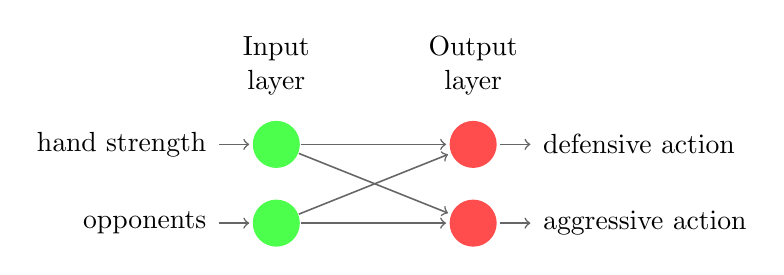
\begin{tikzpicture}[shorten >=1pt,->,line width=0.2mm,draw=black!60, node distance=\layersep]
    \tikzstyle{every pin edge}=[<-,shorten <=1pt]
    \tikzstyle{neuron}=[circle,fill=black!25,minimum size=17pt,inner sep=0pt]
    \tikzstyle{input neuron}=[neuron, fill=green!70];
    \tikzstyle{output neuron}=[neuron, fill=red!70];
    \tikzstyle{hidden neuron}=[neuron, fill=blue!70];
    \tikzstyle{annot} = [text width=4em, text centered]

    % Draw the input layer nodes
    \node[input neuron, pin=left:hand strength] (I-1) at (0,-1) {};
    \node[input neuron, pin=left:opponents] (I-2) at (0,-2) {};

    % Draw the output layer node
    \node[output neuron,pin={[pin edge={->}]right:defensive action}] (O-1) at (\layersep,-1) {};
    \node[output neuron,pin={[pin edge={->}]right:aggressive action}] (O-2) at (\layersep,-2) {};

    % Connect every node in the input layer with every node in the
    % hidden layer.
    \path (I-1) edge (O-1);
    \path (I-2) edge (O-1);
    \path (I-1) edge (O-2);
    \path (I-2) edge (O-2);

    % Annotate the layers
    \node[annot,above of=I-1, node distance=1cm] (il) {Input layer};
    \node[annot,right of=il] {Output layer};
\end{tikzpicture}
\caption{First ANN design. \label{fig:nn1}}
\end{figure}

The first input is the hand strength. We use the calculator from chapter \ref{sec:part1} to calculate the probability of winning against a single opponent. The reason we always find the probability against a single opponent is because the probability of winning decreases drastically as the number of opponents increases. In the start of a round all players are still in the game but it is unlikely that every player will make it to the showdown.

To avoid calculating a hand strength that will most likely become outdated as players fold, we instead find an absolute hand strength that is not affected by the number of players. Instead we give the number of players to the ANN and let the ANN find the pattern between the number of players and the actions.

We define an absolute hand strength as the hand strength versus one opponent. Using an absolute hand strength makes it easier to compare the hands strengths in situations with different numbers of players. \\

Since the inputs in the ANN has to be between zero and one we will have to normalize some of our input data.

The first input is the hand strength found using the calculator. It is already between zero and one so no normalisation is needed. 

The second input is the number of opponents. The second input is normalized as 

\[I_{2} = \frac{Opp}{Opp_{max}}\,.\]

Here, $Opp$ is the number of opponents and $Opp_{max}$ is the maximum number of opponents (in our case nine).



\subsubsection{Test of ANN 1}
\label{sec:ann-test1}
For this test the dataset only includes the normalized data about the strength of the hand of the player, the community cards and the number of opponents.

To find the TNE of the perceptron described in section \ref{sec:design1}, we train it using the dataset. The graph seen in figure \ref{fig:tneg1} displays the TNE through each iteration of the training. From the graph we can see, that the TNE does not get any lower than $\sim$19,9 \%.

\begin{figure}[H]
  \center
    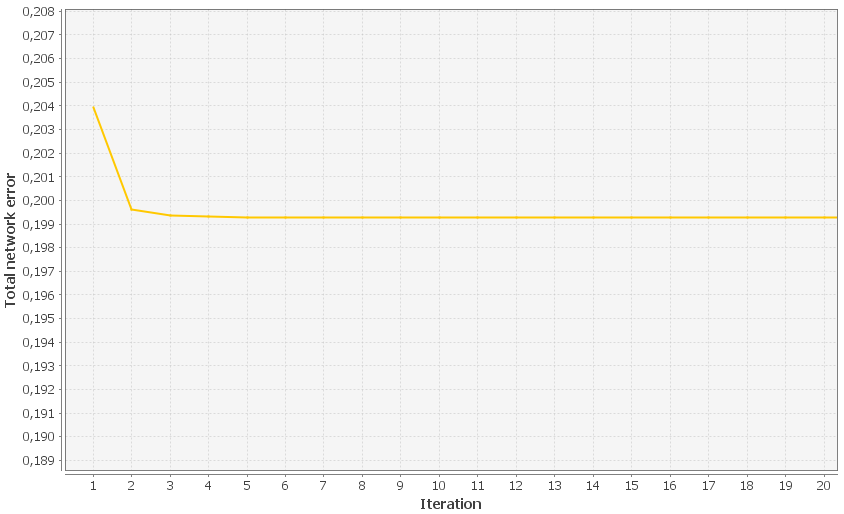
\includegraphics[scale=0.6]{images/nn/default-nn1-err.png}
  \caption{TNE graph from training the first ANN.\label{fig:tneg1}}
\end{figure}


In order for a perceptron to be accurate the data have to be linear separable as shown in figure \ref{fig:ls-example}. This means that the outcomes can be separated by a single straight line if they are inserted in a graph. 

\begin{centering}
\begin{figure}
  \begin{subfigure}[b]{0.4\textwidth}
    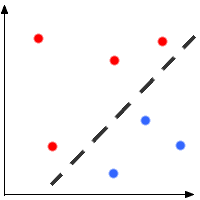
\includegraphics[width=\textwidth]{images/nn/separable.png}
    \caption{Linear separable data.}
  \end{subfigure}
  \hspace{12mm}
  \begin{subfigure}[b]{0.4\textwidth}
    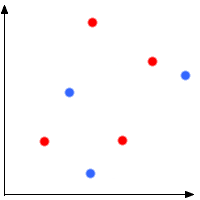
\includegraphics[width=\textwidth]{images/nn/non-separable.png}
    \caption{Non linear separable data.}
  \end{subfigure}
  \caption{Example of linear separable data.\label{fig:ls-example}}
\end{figure}
\end{centering}

We plot some of the data in figure \ref{fig:linear-separable} to see if it is linear separable.  The figure clearly shows that the data is not linear separable and therefore a single perceptron will not work.


\begin{figure}[H]
  \center
    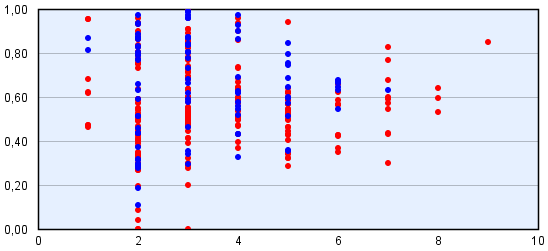
\includegraphics[scale=0.8]{images/nn/default-nn1-plot.png}
  \caption{Distribution of actions. The x-axis  the number of opponents and the y-axis is the hand strength. Aggressive actions are indicated by red dots and defensive actions by blue dots. \label{fig:linear-separable}}
\end{figure}

\subsubsection{ANN 2}
\label{sec:design2}
As we would like the TNE to be equal to or less than five percent. We instead design a multilayer perceptron (MLP) with five inputs, in the hopes or lowering the TNE, see figure \ref{fig:nn2}.

The MLP is taking the same inputs as the perceptron from section \ref{sec:design1}, and three additional inputs: The chips of the player, the cost for the player to call, and the pot. Furthermore this ANN has two hidden neurons. We normalize the three new inputs as: 

\[I_{3} = \frac{chips}{chips_{total}}\] 
\[I_{4} = \frac{cost}{chips_{total}}\]
\[I_{5} = \frac{pot}{chips_{total}}\]

Here $chips$ is the APC's chips, $cost$ is how many chips it costs to call, $pot$ is the amount of chips at stake, and $chips_{total}$ is the total amount of chips in the game, including the pot and the bets.


\def\layersep{2.5cm}

\begin{figure}[H]
\center
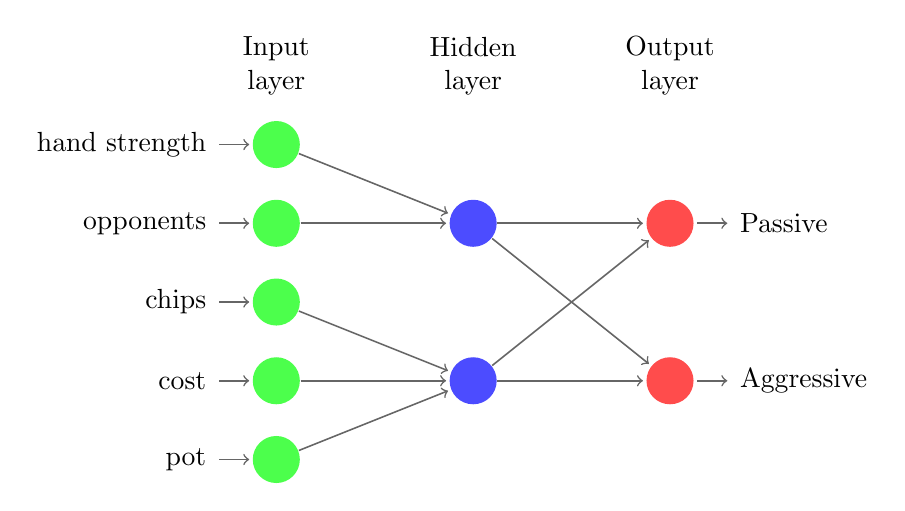
\begin{tikzpicture}[shorten >=1pt,->,line width=0.2mm,draw=black!60, node distance=\layersep]
    \tikzstyle{every pin edge}=[<-,shorten <=1pt]
    \tikzstyle{neuron}=[circle,fill=black!25,minimum size=17pt,inner sep=0pt]
    \tikzstyle{input neuron}=[neuron, fill=green!70];
    \tikzstyle{output neuron}=[neuron, fill=red!70];
    \tikzstyle{hidden neuron}=[neuron, fill=blue!70];
    \tikzstyle{annot} = [text width=4em, text centered]

    % Draw the input layer nodes
    %\foreach \name / \y in {1,...,4}
    % This is the same as writing \foreach \name / \y in {1/1,2/2,3/3,4/4}
    \node[input neuron, pin=left:hand strength] (I-1) at (0,-1) {};
    \node[input neuron, pin=left:opponents] (I-2) at (0,-2) {};
    \node[input neuron, pin=left:chips] (I-3) at (0,-3) {};
    \node[input neuron, pin=left:cost] (I-4) at (0,-4) {};
    \node[input neuron, pin=left:pot] (I-5) at (0,-5) {};

    % Draw the hidden layer nodes
    \node[hidden neuron] (H-1) at (\layersep,-2) {};
    \node[hidden neuron] (H-2) at (\layersep,-4) {};

    % Draw the output layer node
    \node[output neuron,pin={[pin edge={->}]right:Passive}] (O-1) at (2*\layersep,-2) {};
    \node[output neuron,pin={[pin edge={->}]right:Aggressive}] (O-2) at (2*\layersep,-4) {};

    % Connect every node in the input layer with every node in the
    % hidden layer.
    \path (I-1) edge (H-1);
    \path (I-2) edge (H-1);
    \path (I-3) edge (H-2);
    \path (I-4) edge (H-2);
    \path (I-5) edge (H-2);
    
    % Connect every node in the hidden layer with the output layer
    \path (H-1) edge (O-1);
    \path (H-1) edge (O-2);
    \path (H-2) edge (O-1);
    \path (H-2) edge (O-2);

    % Annotate the layers
    \node[annot,above of=I-1, node distance=1cm] (il) {Input layer};
    \node[annot,right of=il] (hl) {Hidden layer};
    \node[annot,right of=hl] {Output layer};
\end{tikzpicture}
\caption{Second ANN design. \label{fig:nn2}}
\end{figure}


\subsubsection{Test of ANN 2}
\label{sec:ann-test2}
For this test the dataset also includes the normalised data about chips, cost and pot.

We train the MLP and get the TNE graph shown in figure \ref{fig:tneg2}.

\begin{figure}[H]
  \center
    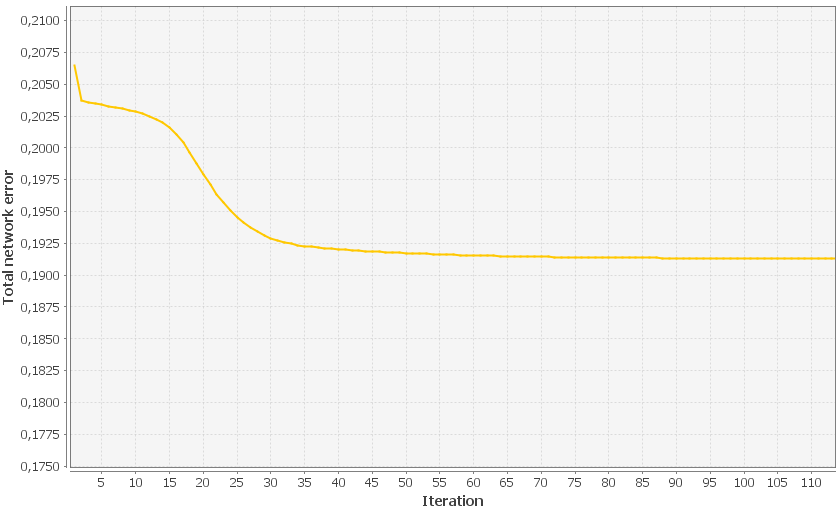
\includegraphics[scale=0.6]{images/nn/default-nn2-err.png}
  \caption{TNE graph from training the second ANN.\label{fig:tneg2}}
\end{figure}

From the test in this section, we can see that the TNE does not get lower than $\sim$19,1 \%. 


We believe that the reason the second ANN did not have a lower TNE is because the data is found from random players. Each player may have a different strategy resulting in different actions. This will make it hard for an ANN to find a pattern. 

There is a small improvement compared to the first ANN in the terms of TNE. It might be a small improvement but perhaps this is the right direction that we are heading.



\subsubsection{ANN 3}
\label{sec:design3}
For our third ANN we use the same structure as the second ANN, see figure \ref{fig:nn2}. Instead of collecting data from random players, we use data of a single player in all games where the player is relevant. This hopefully results in the ANN being able to recognize a pattern in the players strategy.

\subsubsection{Test of ANN 3}
\label{sec:ann-test3}
For this test the dataset contains the same data as the previous test but all data is found for a single player. We try to find the TNE for three different players to see if this makes the ANN more accurate. The players we test are JimR, mayor, and PokiSimA.

For each player we train the MLP from \ref{sec:design2} and find the TNE. The results are shown in table \ref{tab:tneg3}.

\vspace{4mm}
\begin{table}[H]
\center
\begin{tabular}{ | l | l |}
  \hline
  player & TNE (\%) \\
  \hline
  JimR & $\sim$18,7 \\
  mayor & $\sim$14,5 \\
  PokiSimA & $\sim$21,1 \\
  \hline
\end{tabular}
\caption{TNE from training the ANN with different player data.\label{tab:tneg3}}
\end{table}
\vspace{4mm}

There is a rule of thumb when determine the number of hidden neurons that the number of hidden neurons should be between the number of inputs and the number of outputs,
Therefore to further test the ANN we try to test it using different numbers of hidden neurons within that range. We construct three new ANN's with two, three, four, and five hidden neurons. The TNE's can be seen in table \ref{tab:tneg4}. 

The number of hidden neurons does not seem to make the overall TNE get any lower.

\vspace{4mm}
\begin{table}[H]
\center
\begin{tabular}{ | l | l | l | l | }
  \hline
  \#hidden neurons & JimR's TNE (\%) & mayor's TNE (\%) & PokiSimA's TNE (\%) \\
  \hline
  2 & $\sim$19,4 & $\sim$14,5 & $\sim$21,1 \\
  3 & $\sim$19,5 & $\sim$14,0 & $\sim$20,9 \\
  4 & $\sim$19,6 & $\sim$14,2 & $\sim$21,0 \\
  5 & $\sim$19,1 & $\sim$15,0 & $\sim$21,1 \\
  \hline
\end{tabular}
\caption{TNE from training ANN's with different numbers of hidden neurons.\label{tab:tneg4}}
\end{table}
\vspace{4mm}

The tests in this section shows that the TNE varies quite a bit between the players. The higher the TNE are the harder the player is to predict. Because poker is a game of deception, a player will often try to misguide the opponents by making illogical choices. This makes it hard for the ANN to figure out the players strategy.
From this we can tell that mayor is probably more predictable compared to the two other players examined. Therefore mayor is the most preferable player when it comes to the success of learning a players strategy.


\begin{figure}[H]
  \center
    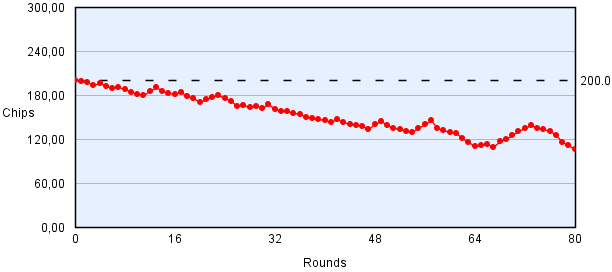
\includegraphics[scale=0.6]{images/nn/finaltest.png}
  \caption{Graph of the profits change throughout the game\label{fig:finaltest}}
\end{figure}

To further test whether or not the ANN can make profitable choices based on the training with the data from the player mayor, we choose to use a test-bed for poker bots called Poker Genius. Here we are able to test the ANN against the poker bots of Poker Genius. We manually recreated the choices the ANN made against the poker bots of Poker Genius because we did not manage to make APC work for Poker Genius. As shown in figure \ref{fig:finaltest} it is clear that the ANN is not able to compete on the same level as the poker bots from Poker Genius.


\subsection{Discussion}
In this chapter we develop a default strategy by implementing an algorithm. We use ANN's to observe the actions of players in order to learn their strategy. We ran into a few problems when implementing the ANN.\\

The first problem is related to the data we use. The problem is that  the data is not complete since we do not have the data about the hole cards of the players who fold. This means that we can not learn the APC when to fold, as we have no input for the hole cards. 

If we want to observe a player and learn the strategy behind the players actions, we need to know the hole cards of the player. To solve this we need to find a new dataset with no hidden information about the player(s) we want the APC to observe.

Additionally, since we get the results as an action (defensive or aggressive), The expected results of each output is either zero or one, due to the limitation of possible actions. Zero or one are the two extremes and therefore it can be hard for the ANN to find an approximation. 

Another problem we encountered was defining our requirements for the ANN. We do not know what TNE is realistic for an ANN for poker and our requirement of a TNE of five percent or less may be unrealistic. It would have been better set the requirement in regards to performance against other poker bots. For instance, a requirement could have been that the APC should have more chips than the test bot after playing a game of 200 rounds. \\

Learning a default strategy based on random players in random rounds was not a good solution. However we were not able to retrieve any game data from professional poker players.
An alternative method would be to choose the most successful player in the dataset, but that raises the issue that just because a players strategy is good against one strategy does not make it good against another.
Another issue is that in order for a player to be successful the player has to be good at adapting to the opponents strategy. This would mean that the ANN would have a hard time learning the strategy of the player, as the player may change the strategy or may use a completely different strategy if given other opponents. Our data was tracked for a game where players can join and leave as they please. It is therefore very likely that the players we observed changed strategy during the game. 

The ANN were not able to make profitable choices when playing against the poker bots of Poker Genius. We believe the main reason for the bad performance was the fact that the APC never learned when to fold. We believe that this method for developing a default strategy could have worked better if we were to get data from poker games where at least one of the players had no hidden information.

\subsection{Conclusion}
In this chapter we answer problem statement 2:

\vspace{4mm}
\begin{statementBox2}{Problem statement 2}
How can we develop a default strategy for APC without having information about the playing style of the opponents?
\end{statementBox2}
\vspace{4mm}

We develop the strategy by creating different ANN's and train them using data from real-life poker games.

The tests were partly successful, as they show that we in fact were able to train an ANN to recognise the strategy of the players. We created several TNE graphs that display that the ANN becomes smarter as the training progresses. Although we did not manage to design an ANN that could learn the strategy of a player well enough.

By finding a more relevant dataset using only one players actions. We managed to get an absolute improvement of the TNE of $\sim$6~\% which is a relative improvement of $\sim$30~\%.

Our best ANN design takes five inputs (hand strength, number of opponents, chips, cost, and pot) and produce two outputs (whether to play defensive and whether to play aggressive). 

We tested it using three randomly picked players. We got an TNE of $\sim$14~\%, $\sim$19~\%, and $\sim$21~\% for each of the players respectively.

We also tested the APC against a simple poker bot, and the APC end up losing roughly half its amount of chips in 80 rounds.